\chapter{Risk, Structure, and Repeated Proof: Dana White and the Commercial Mechanics of Scale}

In this School of Hard Knocks interview, curated by LazyingArt LLC, the argument begins with spectacle and only later reveals its machinery. We are first given the scale of Dana White and the UFC, then sent through Beverly Hills to collect a vocabulary of invention, work, compounding, entity structure, deal flow, patents, and belief. Only after that runway does the lecture arrive in Las Vegas, where Dana White turns those scattered mechanisms into a harder doctrine: take risk before responsibility hardens, redesign the product instead of worshiping the incumbent form, prove yourself again each year, and measure progress by whether today beats yesterday.

\section{Opening Scale and the Wager}

The opening claim is not subtle. Dana White is introduced as a legendary entrepreneur, and the UFC is immediately described as a multi-billion-dollar company. That claim functions as a scale marker rather than as a valuation proof, but it matters because it sets the ceiling of the whole discussion before any mechanism is explained.

\begin{equation}
V_{\mathrm{UFC}} \gg \$10^9
\end{equation}

We should read this not as audited finance but as the lecture's opening condition: the enterprise is already so large that any later advice must answer to scale, not merely to hustle. The host then delays the main interview and goes to Beverly Hills. That delay is structural. The lecture wants us to assemble a set of smaller commercial mechanisms before we meet the larger operator who has fused them into a single style of action.

\section{Beverly Hills: Invention, Compounding, and Early Rules}

The first Beverly Hills interview gives us an older entrepreneur who claims invention, sustained labor, a missed Google investment, tax-free bond accumulation, and an industrial real-estate rule. The interview is loose and anecdotal, but the lecture repeatedly pushes it toward a more abstract grammar.

The first formula is not a law of nature but a narrated ratio of temperament:

\begin{equation}
\rho_{\mathrm{effort}} = 0.95,
\qquad
\rho_{\mathrm{luck}} = 0.05.
\end{equation}

That figure is immediately followed by a second contrast: very small missed optionality and much larger later entrepreneurial expenditure.

\begin{equation}
I_{\mathrm{Google,missed}} = \$5{,}000,
\qquad
C_{\mathrm{first\,app}} \approx \$1{,}000{,}000.
\end{equation}

The point is not merely regret. The point is that entrepreneurial life is full of asymmetries that are visible only in retrospect. A tiny investment that never happened sits in memory beside a much larger risk that did happen. The lecture uses that juxtaposition to prepare the next move, which is capital allocation.

The same speaker then gives a bond-versus-stock comparison:

\begin{equation}
r_{\mathrm{stock,claimed}} \approx 12\%,
\qquad
r_{\mathrm{CA\,taxfree}} \approx 5\%,
\qquad
K_0 \approx \$2\times 10^6,
\qquad
K_T \approx \$50\times 10^6.
\end{equation}

We should be careful here. These numbers are part of the spoken account and should be preserved, but they do not force a clean single-rate compound-growth derivation. The lecture's interest is elsewhere. It is contrasting glamour with safety, taxable upside with tax-free steadiness, and a speculative atmosphere with a conservative one.

The second rule in this sequence concerns industrial real estate:

\begin{equation}
d_{\mathrm{down}} = 0.5.
\end{equation}

The oral rule is: buy investment property, put \(50\%\) down, never leverage it, never sell it. The transcript later says that the mortgage goes down while the payments on the property go up. That wording is not precise, but the commercial intuition is clear enough: the debt is amortized while the asset's income or effective value rises. We should preserve the rule without pretending the speaker gave a full real-estate model.

\paragraph{Mechanism.}
The lecture is already separating three things that are often blurred together: the story of getting rich, the claim that one is rich, and the mechanism by which wealth persists. The Beverly Hills prelude matters because it starts this separation early.

\section{Structure Before Scale}

The next pivot is from wealth to protection. The interviewer asks about entity structure and receives a blunt answer: yes, it was a mistake not to begin with an LLC, because liability can reach what should remain personal.

\subsection{Question \& Answer}

\paragraph{Question.}
Was not having an LLC a mistake?

\paragraph{Answer.}
Yes. The interviewer's formulation is practical rather than technical: when a business is sued, one does not want the house, the car, and personal assets exposed to the business shock. The legal shell is therefore presented as a first protection, not as an afterthought.

A schematic way to record the point is the following:

\begin{equation}
\mathcal{A}_{\mathrm{personal}} \not\subset \mathcal{L}_{\mathrm{business}}.
\end{equation}

This is only a note-writer's shorthand. It does not mean that law literally operates by set inclusion; it means that the lecture insists on a barrier between the person and the operating liability.

\begin{figure}[h]
\centering
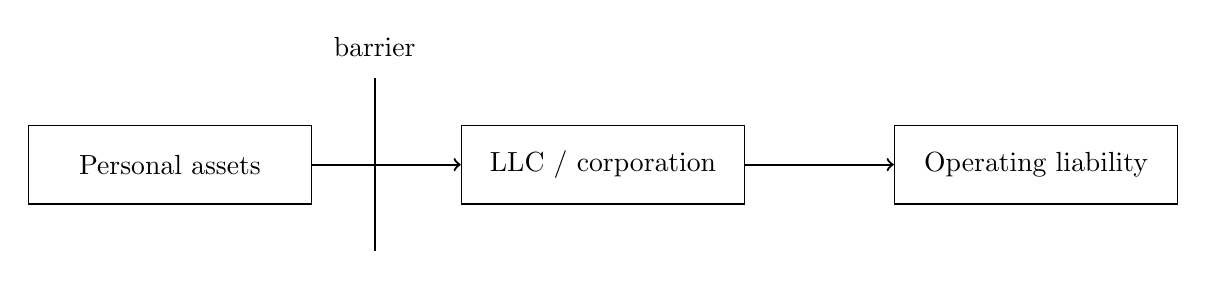
\begin{tikzpicture}[x=1cm,y=1cm]
\node[draw, rectangle, minimum width=3.6cm, minimum height=1cm] (p) at (0,0) {Personal assets};
\node[draw, rectangle, minimum width=3.6cm, minimum height=1cm] (e) at (5.5,0) {LLC / corporation};
\node[draw, rectangle, minimum width=3.6cm, minimum height=1cm] (l) at (11,0) {Operating liability};
\draw[->, thick] (p) -- (e);
\draw[->, thick] (e) -- (l);
\draw[thick] (2.6,-1.1) -- (2.6,1.1);
\node at (2.6,1.5) {barrier};
\end{tikzpicture}
\caption{A transcript-backed schematic of the liability shield. The interview does not provide legal formalism, only the commercial function of the entity boundary.}
\end{figure}

The host then gives a sponsor-shaped expansion of this point. We should keep it in reduced form. Its narrative role is not to replace the guest's lesson but to translate it: too many entrepreneurs build the business first and only later think about the shell that contains it. The lecture wants us to hear this as a foundation problem.

\section{Dealmaking, Patents, and the Propagation of Opportunity}

The second Beverly Hills interview shifts the lecture from protection to acquisition. Jeffrey Phillips gives three related claims: he made a \$48 million commission by putting together two sides of a deal, he owns gaming patents whose use throws off cash, and he believes that once one declares a target loudly enough the surrounding network begins to route opportunities back.

\subsection{Question \& Answer}

\paragraph{Question.}
How does a \$48 million commission happen?

\paragraph{Answer.}
Not, in this telling, by being the smartest man in the room in the academic sense. It happens by overhearing, connecting a seller to a buyer, and standing at the point where information becomes a transaction.

The lecture gives us enough numerical content for a worked example.

\paragraph{Worked example: the casino transaction.}
\begin{align}
D_{\mathrm{casino}} &\approx \$450\times 10^6, \\
C_{\mathrm{commission}} &\approx \$48\times 10^6, \\
\alpha_{\mathrm{commission}}
&=
\frac{C_{\mathrm{commission}}}{D_{\mathrm{casino}}}
\approx
\frac{48}{450}
\approx
0.107.
\end{align}

So the implied take is about \(10.7\%\). This percentage is not stated in the interview; it is our arithmetic on the spoken numbers. The lecture uses the numbers not to define a universal fee schedule but to dramatize the economics of intermediary position.

The same speaker gives a billion-scale valuation marker:

\begin{equation}
V_{\mathrm{gaming\,company}} \approx \$1.2\times 10^9,
\qquad
a_{\mathrm{millionaire}} \approx 27,
\qquad
a_{\mathrm{current}} \approx 58.
\end{equation}

Then comes the patent mechanism. The specific claim is that he owns the patents to blackjack bonus-round structures and gets paid when people play and lose. Since no royalty formula is given, the cleanest formalization is only proportional:

\begin{equation}
R_t \propto Q_t,
\end{equation}

where \(Q_t\) is play volume and \(R_t\) is the resulting revenue to the right-holder. The important point is ownership of the rule-set, not labor inside each individual game.

The most metaphysical part of the interview is also commercially useful. Jeffrey says that if he declares that he will own a building, the universe opens; in practical terms, one person hears, another knows the owner, and an introduction is made. We may write the sequence as

\begin{equation}
T_{\mathrm{declared}} \to N(T) \to I_{\mathrm{intro}} \to D_{\mathrm{deal}}.
\end{equation}

Here the notation is only mnemonic. The lecture is not claiming a deterministic law. It is claiming that public intention changes network visibility, and visibility changes the chance of a matching introduction.

\begin{figure}[h]
\centering
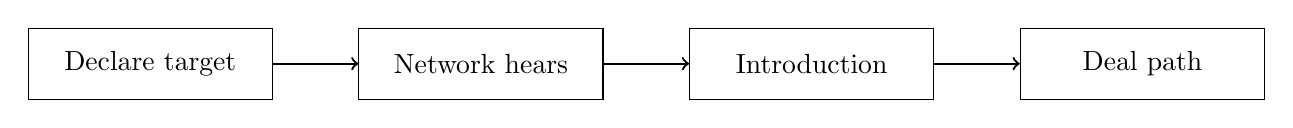
\begin{tikzpicture}[x=1cm,y=1cm]
\node[draw, rectangle, minimum width=3.1cm, minimum height=0.9cm] (t) at (0,0) {Declare target};
\node[draw, rectangle, minimum width=3.1cm, minimum height=0.9cm] (n) at (4.2,0) {Network hears};
\node[draw, rectangle, minimum width=3.1cm, minimum height=0.9cm] (i) at (8.4,0) {Introduction};
\node[draw, rectangle, minimum width=3.1cm, minimum height=0.9cm] (d) at (12.6,0) {Deal path};
\draw[->, thick] (t) -- (n);
\draw[->, thick] (n) -- (i);
\draw[->, thick] (i) -- (d);
\end{tikzpicture}
\caption{The lecture's social propagation mechanism, reconstructed from the transcript. Public intention is converted into network visibility, then into contact, then into deal possibility.}
\end{figure}

\section{Dana White and the Product Insight}

Only now do we arrive in Las Vegas. The visit to the UFC Performance Institute and the host's full-circle remarks are not expendable scenery. They create a threshold. The interview must feel earned before it becomes analytical.

Dana White begins before the UFC, with the simple recognition that the life in front of him was not his life. The important line is not grand destiny but mismatch: this isn't me. From there he gives the lecture's risk timing rule. When one is young, before children and heavier responsibilities arrive, one should take the risk because one can still go back if the gamble fails.

The key commercial question is then asked directly.

\subsection{Question \& Answer}

\paragraph{Question.}
What did he see in the UFC that others did not?

\paragraph{Answer.}
He and his partners loved the storylines, thought the fighting was more exciting than boxing, and believed they could keep what they loved about boxing while removing what they hated.

The cleanest symbolic summary is therefore:

\begin{equation}
\text{UFC product}
\approx
\text{boxing}_{\mathrm{loved}}
-
\text{boxing}_{\mathrm{hated}}
+
\text{MMA intensity/storylines}.
\end{equation}

This is not Dana White's notation; it is a compact statement of the product logic. The lecture's conception of disruption is not creation ex nihilo. It is selective subtraction, selective retention, and a higher-energy package. That is why the later advice to entrepreneurs is not merely ``be different.'' It is: go in and break rules that are old only because people stopped examining them.

\paragraph{A more precise reading.}
The lecture is careful here. Dana White does not say that incumbents were stupid. He says they were trapped by habit. The difference matters. Habit makes existing rules feel like laws of nature. The interview insists they are usually only inherited conventions.

\section{Repeated Proof, Loyalty, and Crisis}

The next move is subtle and important. Once the lecture has shown product insight, it refuses to let success harden into a victory lap. Dana White says that even after a new deal with Paramount, he goes into January on a fresh slate and has to prove himself again.

\subsection{Question \& Answer}

\paragraph{Question.}
What does it mean to keep proving yourself after you have already won?

\paragraph{Answer.}
It means that scale does not cancel recurrence. A big deal enlarges the platform, but it does not abolish next year's burden.

The largest raw number in the interview appears here:

\begin{equation}
D_{\mathrm{Paramount}} = \$7.7\times 10^9.
\end{equation}

But the doctrinal point is not the size of the contract. The doctrinal point is the reset. The lecture wants us to reject the fantasy of final arrival. White's Italy ritual each Christmas serves exactly this purpose: withdraw, recover, and return hungry. One does not remain at the summit by admiring the summit.

Competition is treated in the same spirit. He says he loves competition, and he explicitly frames the world of business as a fight in which there are winners and losers. Here the lecture risks sounding merely warlike, but it immediately complicates itself by asking about loyalty and keeping one's word.

The COVID sequence is crucial. White says he did not want to lay off employees when revenue froze. He casts the company as a battleship: either all go down together or not at all. Then, when ordinary venues were blocked, he did not surrender the business; he redesigned the distribution path.

\begin{figure}[h]
\centering
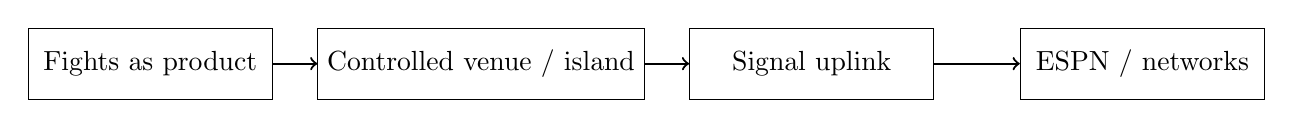
\begin{tikzpicture}[x=1cm,y=1cm]
\node[draw, rectangle, minimum width=3.1cm, minimum height=0.9cm] (p) at (0,0) {Fights as product};
\node[draw, rectangle, minimum width=3.1cm, minimum height=0.9cm] (v) at (4.2,0) {Controlled venue / island};
\node[draw, rectangle, minimum width=3.1cm, minimum height=0.9cm] (s) at (8.4,0) {Signal uplink};
\node[draw, rectangle, minimum width=3.1cm, minimum height=0.9cm] (n) at (12.6,0) {ESPN / networks};
\draw[->, thick] (p) -- (v);
\draw[->, thick] (v) -- (s);
\draw[->, thick] (s) -- (n);
\end{tikzpicture}
\caption{The COVID workaround as a distribution diagram reconstructed from the transcript. The lecture's claim is that the product needed a new route to the audience when the ordinary route was blocked.}
\end{figure}

The line ``don't tell me something can't be done'' sits exactly here, and now we can see why. It is not vague optimism. It is logistics plus refusal. He had a product, a venue problem, a transmission problem, and counterparties who needed the content. The solution is therefore not mystical. It is entrepreneurial geometry under constraint.

\section{Consistency and the Daily Update Rule}

The final movement compresses the entire interview into a recurrence relation. When asked what the most successful people have in common, White answers: consistency. Then he sharpens it. To have consistency, one must also have drive.

The lecture next turns generational, but the deeper point is not sociological. It is operational. Standing out is easier when others are vague, unserious, under-reinvested, or unwilling to endure repeated effort. This is why White immediately praises the visible labor behind influencing, touring, and reinvesting in oneself. The same structure appears again: glamour outside, machinery underneath.

At the end the interview becomes almost axiomatic. White gives the sentence by which he lives: every day we try to be better than yesterday, whether in business, in our bodies, or in our relationships.

\subsection{Question \& Answer}

\paragraph{Question.}
How do we beat yesterday?

\paragraph{Answer.}
Not by a mystical leap, and not by a once-for-all breakthrough, but by imposing a simple order relation on successive days.

\begin{equation}
X_{t+1} > X_t.
\end{equation}

Here \(X_t\) is intentionally broad. The interview itself broadens it. The variable may represent business execution, physical condition, personal conduct, or relational steadiness. The key is that the lecture ends with an update rule rather than a slogan.

\begin{definition}
Let \(X_t\) denote the state of one chosen domain on day \(t\): business, fitness, relationships, or disciplined conduct. The lecture's final command is to prefer trajectories for which \(X_{t+1} > X_t\) whenever comparison is meaningful.
\end{definition}

This is the chapter's hardest-won abstraction. It would be easy to hear only the aggressive tone: no mercy, competition, war, jealousy. But the mathematical spine underneath is more sober. The lecture values recurrence over declaration. If the day does not improve the state, then the rhetoric has outrun the mechanism.

\section{Summary}

The lecture begins with scale and ends with recurrence. Between those two poles it passes through invention, missed asymmetry, conservative compounding, real-estate rules, entity protection, intermediary economics, patent cash flow, public intention as network activation, product redesign, repeated proof, and crisis logistics. Dana White enters late because the Beverly Hills prelude is doing preparatory work: it teaches us to separate anecdote from mechanism.

The final doctrine is therefore not one doctrine but a sequence. First, take risk before the cost of risk rises. Second, protect the shell before scale arrives. Third, own position, rights, or narrative leverage rather than mere activity. Fourth, redesign the product by keeping what is loved and cutting what is stale. Fifth, after every victory, begin again. And sixth, if we need one formula to hold the whole chapter together, it is the smallest one and the hardest one:

\begin{equation}
X_{t+1} > X_t.
\end{equation}

That is the lecture's last compression of wealth, entrepreneurship, and commercial character into a single daily test.